\documentclass{scrartcl}
\usepackage[margin=3cm]{geometry}
\usepackage{amsmath}
\usepackage{amssymb}
\usepackage{amsthm}
\usepackage{blindtext}
\usepackage{datetime}
\usepackage{fontspec}
\usepackage{float}
\usepackage{graphicx}
\usepackage{kotex}
\usepackage[lighttt]{lmodern}
\usepackage{listings}
\usepackage{mathrsfs}
\usepackage{mathtools}
\usepackage{pgf,tikz,pgfplots}

\pgfplotsset{compat=1.15}
\usetikzlibrary{arrows}
\newtheorem{theorem}{Theorem}

\lstset{
  numbers=none, frame=single, showspaces=false,
  showstringspaces=false, showtabs=false, breaklines=true, showlines=true,
  breakatwhitespace=true, basicstyle=\ttfamily, keywordstyle=\bfseries, basewidth=0.5em
}

\setmainhangulfont{Noto Serif CJK KR}[
  UprightFont=* Light, BoldFont=* Bold,
  Script=Hangul, Language=Korean, AutoFakeSlant,
]
\setsanshangulfont{Noto Sans CJK KR}[
  UprightFont=* DemiLight, BoldFont=* Medium,
  Script=Hangul, Language=Korean
]
\setmathhangulfont{Noto Sans CJK KR}[
  SizeFeatures={
    {Size=-6,  Font=* Medium},
    {Size=6-9, Font=*},
    {Size=9-,  Font=* DemiLight},
  },
  Script=Hangul, Language=Korean
]
\title{디지털시스템설계 Lab 2}
\author{손량(20220323)}
\date{Last compiled on: \today, \currenttime}

\newcommand{\un}[1]{\ensuremath{\ \mathrm{#1}}}

\begin{document}
\maketitle

\section{개요}
이 실험에서는 강의 시간에 배운 Karnaugh map 등을 이용하여 boolean expression을 단순화하는 방법과, 그 효과에 대해서 실습한다.

\section{이론적 배경}

\subsection{Karnaugh Map}
불 대수식을 sum of products 형식으로 최대한 간단하게 표현하는 시각적인 기법이다. Karnaugh map을 사용하면 2-level circuit으로 논리 식을 나타낼 수 있다.

\subsection{2-bit Magnitude Comparator}
서로 다른 2비트 숫자 \(A\), \(B\)가 주어졌을 때, 둘의 대소 관계를 출력하는 논리 회로이다. \(A\)와 \(B\)를 받는 입력 4개와, \(A > B\), \(A = B\), \(A < B\) 각각에 해당하는 출력 3개로 이루어져 있다.

\section{실험 준비}
우선 \(A = B\) 일 때의 truth table은 다음과 같다.
\begin{table}[H]
  \centering
  \begin{tabular}{|cccc|c|}
  \hline
  \(A_0\) & \(A_1\) & \(B_0\) & \(B_1\) & Out \\ \hline
  0       & 0       & 0       & 0       & 1   \\
  0       & 0       & 0       & 1       & 0   \\
  0       & 0       & 1       & 0       & 0   \\
  0       & 0       & 1       & 1       & 0   \\
  0       & 1       & 0       & 0       & 0   \\
  0       & 1       & 0       & 1       & 1   \\
  0       & 1       & 1       & 0       & 0   \\
  0       & 1       & 1       & 1       & 0   \\
  1       & 0       & 0       & 0       & 0   \\
  1       & 0       & 0       & 1       & 0   \\
  1       & 0       & 1       & 0       & 1   \\
  1       & 0       & 1       & 1       & 0   \\
  1       & 1       & 0       & 0       & 0   \\
  1       & 1       & 0       & 1       & 0   \\
  1       & 1       & 1       & 0       & 0   \\
  1       & 1       & 1       & 1       & 1   \\ \hline
  \end{tabular}
\end{table}

Minterm expansion을 통해 그대로 나타낸 결과는 다음과 같다.
\begin{align*}
  F(A_0, A_1, B_0, B_1) &= \sum m(0, 5, 10, 15) \\
                        &= A_0' A_1' B_0' B_1' + A_0' A_1 B_0' B_1 + A_0 A_1' B_0 B_1' + A_0 A_1 B_0 B_1
\end{align*}
K-map을 그려보면 다음과 같다.
\begin{figure}[H]
  \centering
  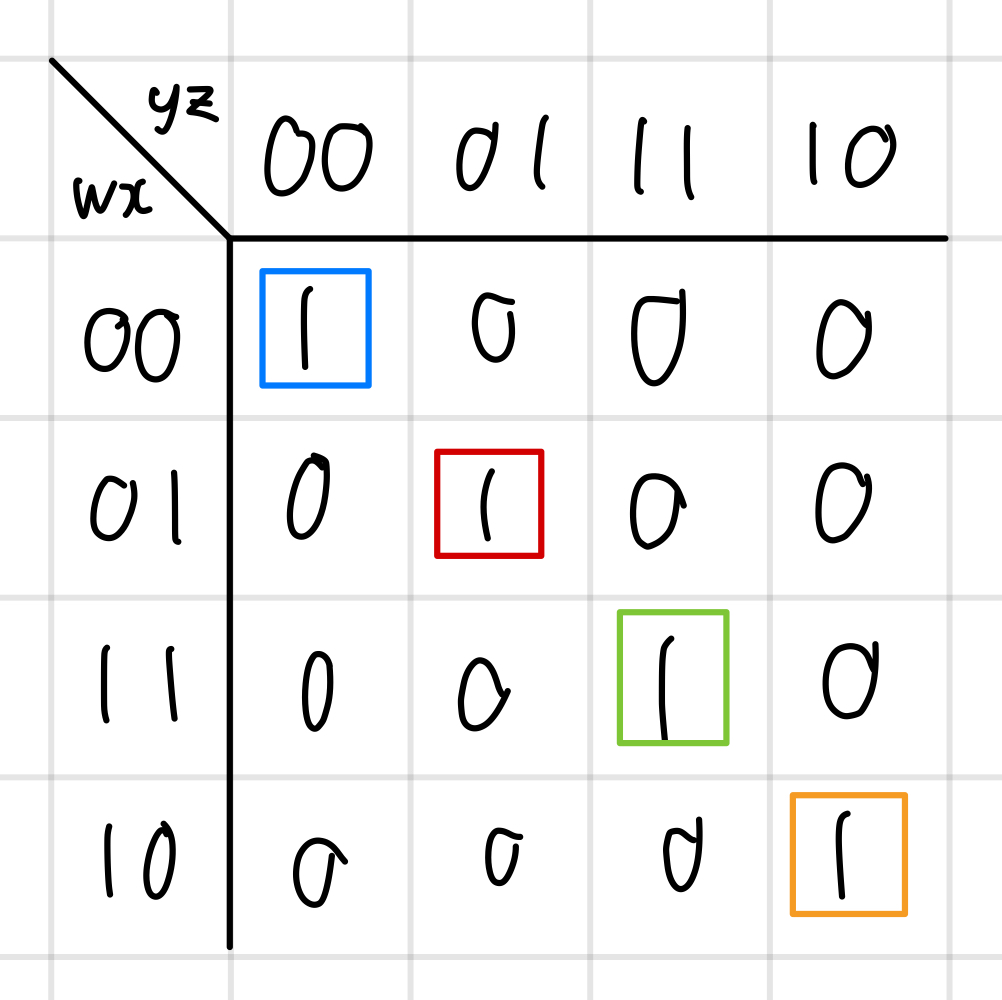
\includegraphics[width=0.4\linewidth]{EQ_KM}
\end{figure}
모든 prime implicant가 1개의 1만 커버하기 떄문에, simplification을 더 이상 할 수 없다.

\(A < B\)에서의 truth table은 다음과 같다.
\begin{table}[H]
  \centering
  \begin{tabular}{|cccc|c|}
  \hline
  \(A_0\) & \(A_1\) & \(B_0\) & \(B_1\) & Out \\ \hline
  0       & 0       & 0       & 0       & 0   \\
  0       & 0       & 0       & 1       & 1   \\
  0       & 0       & 1       & 0       & 1   \\
  0       & 0       & 1       & 1       & 1   \\
  0       & 1       & 0       & 0       & 0   \\
  0       & 1       & 0       & 1       & 0   \\
  0       & 1       & 1       & 0       & 0   \\
  0       & 1       & 1       & 1       & 1   \\
  1       & 0       & 0       & 0       & 0   \\
  1       & 0       & 0       & 1       & 1   \\
  1       & 0       & 1       & 0       & 0   \\
  1       & 0       & 1       & 1       & 1   \\
  1       & 1       & 0       & 0       & 0   \\
  1       & 1       & 0       & 1       & 0   \\
  1       & 1       & 1       & 0       & 0   \\
  1       & 1       & 1       & 1       & 0   \\ \hline
  \end{tabular}
\end{table}
Minterm expansion을 사용하면 다음과 같다.
\begin{align*}
  F(A_0, A_1, B_0, B_1) &= \sum m(1, 2, 3, 7, 9, 11) \\
                        &= A_0' A_1' B_0' B_1 + A_0' A_1' B_0 B_1' + A_0' A_1' B_0 B_1 + A_0' A_1 B_0 B_1 \\
                        &+ A_0' A_1 B_0 B_1 + A_0 A_1' B_0 B_1
\end{align*}
K-map을 그려보면
\begin{figure}[H]
  \centering
  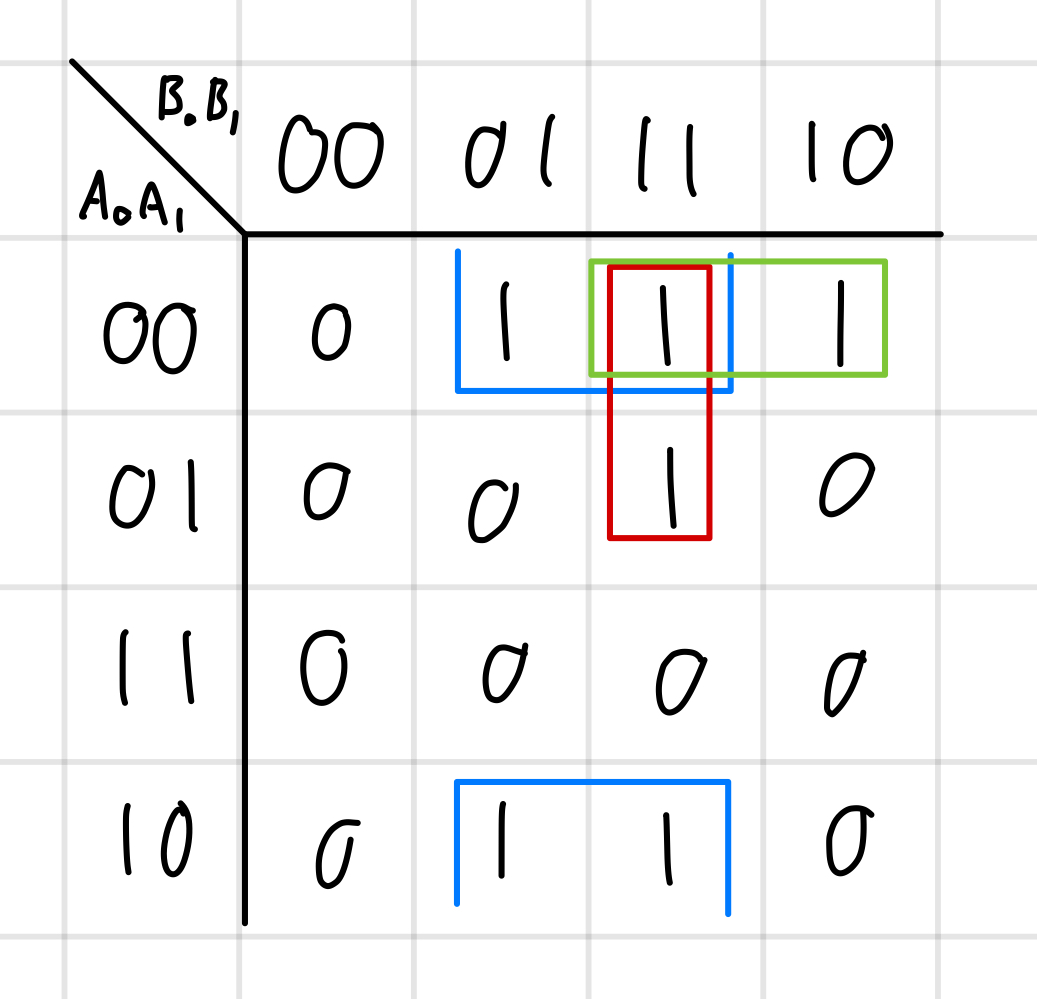
\includegraphics[width=0.4\linewidth]{LT_KM}
\end{figure}
모든 prime implicant가 essential prime implicant임을 알 수 있고, 따라서 각 prime implicant들을 OR로 합쳐서 다음과 같이 simplification 결과를 쓸 수 있다.
\[
  F(A_0, A_1, B_0, B_1) = A_1' B_1 + A_0' B_0 B_1 + A_0' A_1' B_0
\]

\(A > B\)에서의 truth table을 그리면
\begin{table}[H]
  \centering
  \begin{tabular}{|cccc|c|}
  \hline
  \(A_0\) & \(A_1\) & \(B_0\) & \(B_1\) & Out \\ \hline
  0       & 0       & 0       & 0       & 0   \\
  0       & 0       & 0       & 1       & 0   \\
  0       & 0       & 1       & 0       & 0   \\
  0       & 0       & 1       & 1       & 0   \\
  0       & 1       & 0       & 0       & 1   \\
  0       & 1       & 0       & 1       & 0   \\
  0       & 1       & 1       & 0       & 1   \\
  0       & 1       & 1       & 1       & 0   \\
  1       & 0       & 0       & 0       & 1   \\
  1       & 0       & 0       & 1       & 0   \\
  1       & 0       & 1       & 0       & 0   \\
  1       & 0       & 1       & 1       & 0   \\
  1       & 1       & 0       & 0       & 1   \\
  1       & 1       & 0       & 1       & 1   \\
  1       & 1       & 1       & 0       & 1   \\
  1       & 1       & 1       & 1       & 0   \\ \hline
  \end{tabular}
\end{table}

Minterm expansion을 사용하면 다음과 같다.
\begin{align*}
  F(A_0, A_1, B_0, B_1) &= \sum m(4, 6, 8, 12, 13, 14) \\
                        &= A_0' A_1 B_0' B_1' + A_0' A_1 B_0 B_1' + A_0 A_1' B_0' B_1' + A_0 A_1 B_0' B_1' \\
                        &+ A_0 A_1 B_0' B_1 + A_0 A_1 B_0 B_1'
\end{align*}
K-map을 그려보면 다음과 같다.
\begin{figure}[H]
  \centering
  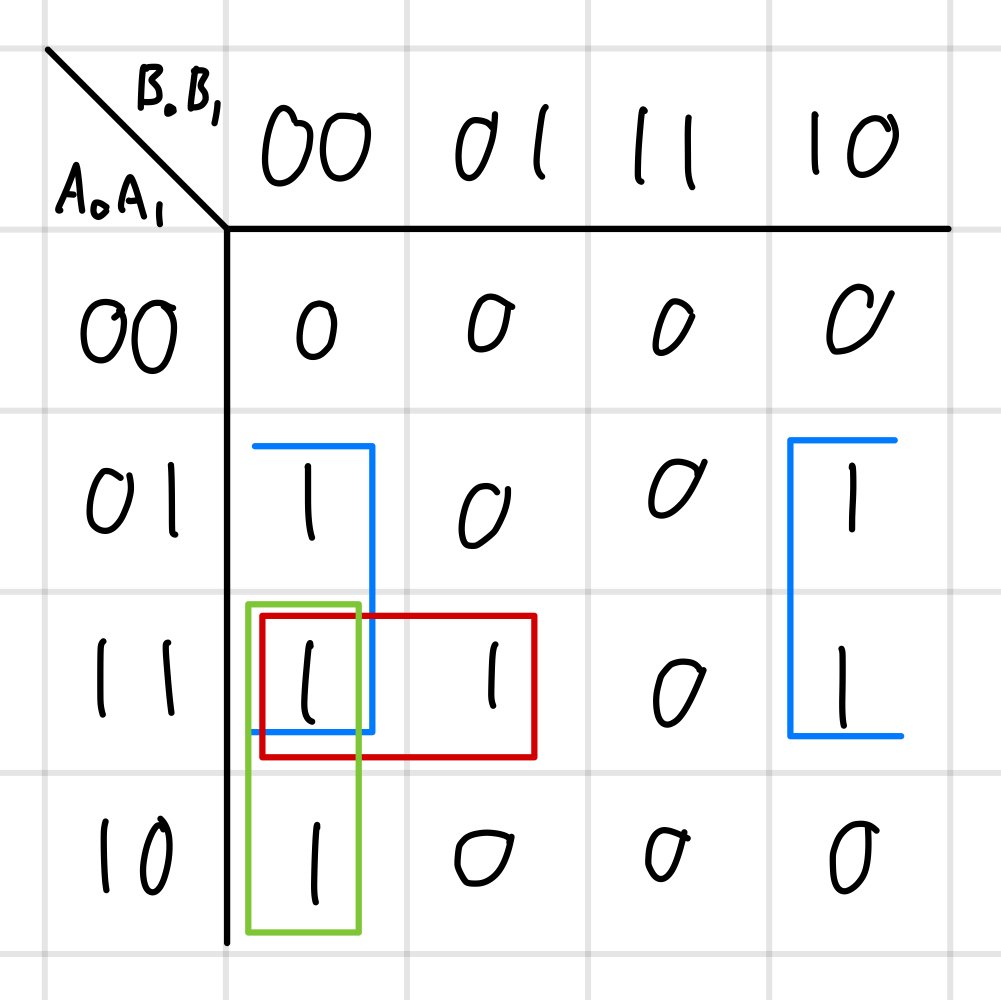
\includegraphics[width=0.4\linewidth]{GT_KM}
\end{figure}
모든 prime implicant가 여기서도 essential prime implicant이고, 앞서와 똑같이 simplification을 하면 다음과 같이 쓸 수 있다.
\[
  F(A_0, A_1, B_0, B_1) = A_1 B_1' + A_0 B_0' B_1' + A_0 A_1 B_0'
\]

\section{실험 결과}
Simplification을 하지 않았을 때의 schematic은 다음과 같다.
\begin{figure}[H]
  \centering
  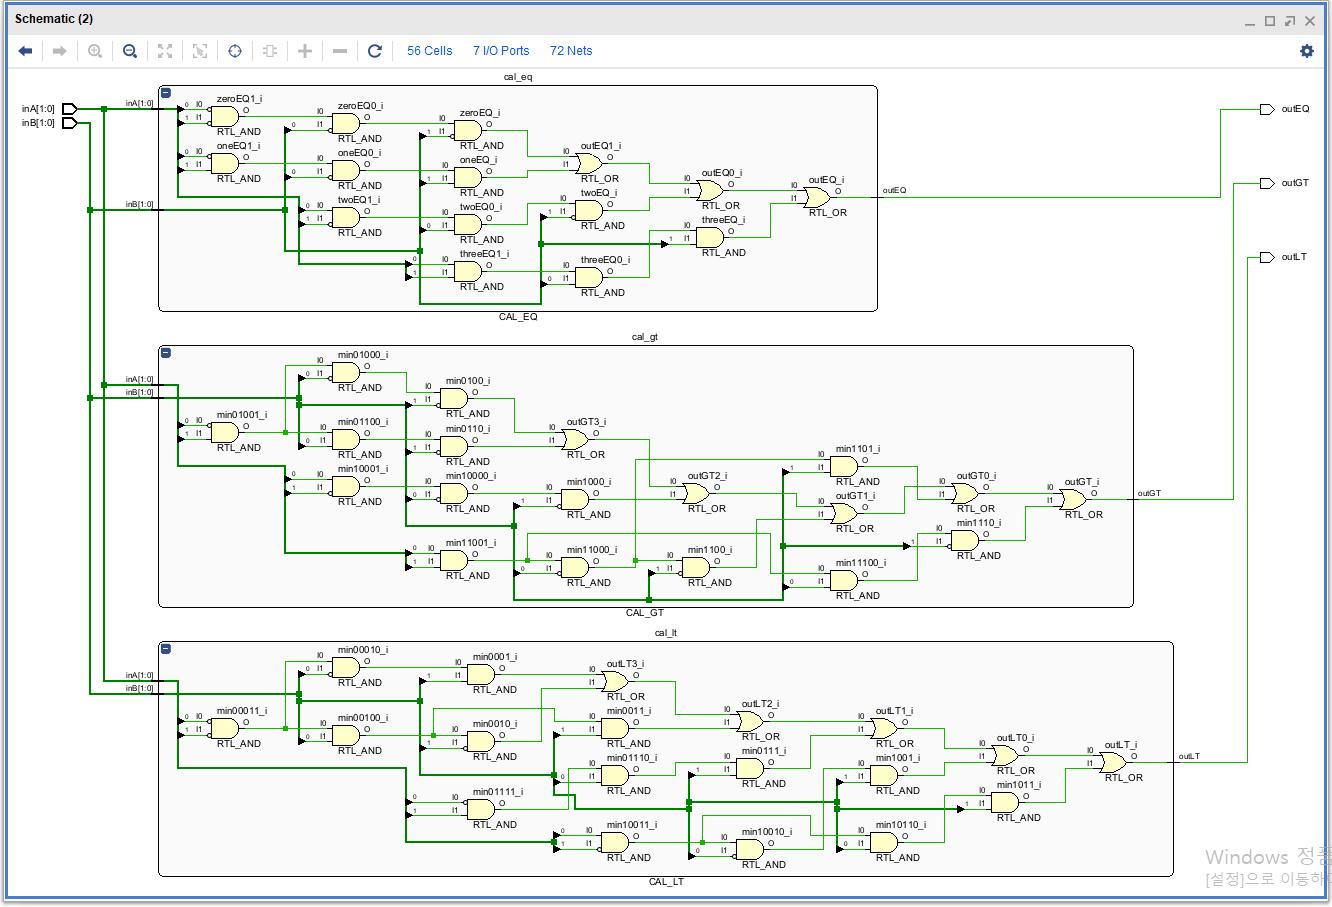
\includegraphics[width=\linewidth]{lab2_1_schematic}
\end{figure}
Netlist는 다음과 같다.
\begin{figure}[H]
  \centering
  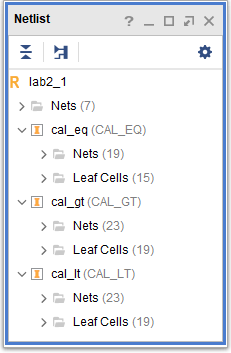
\includegraphics[width=0.4\linewidth]{lab2_1_netlist}
\end{figure}
Simplification을 한 이후의 schematic은 다음과 같다.
\begin{figure}[H]
  \centering
  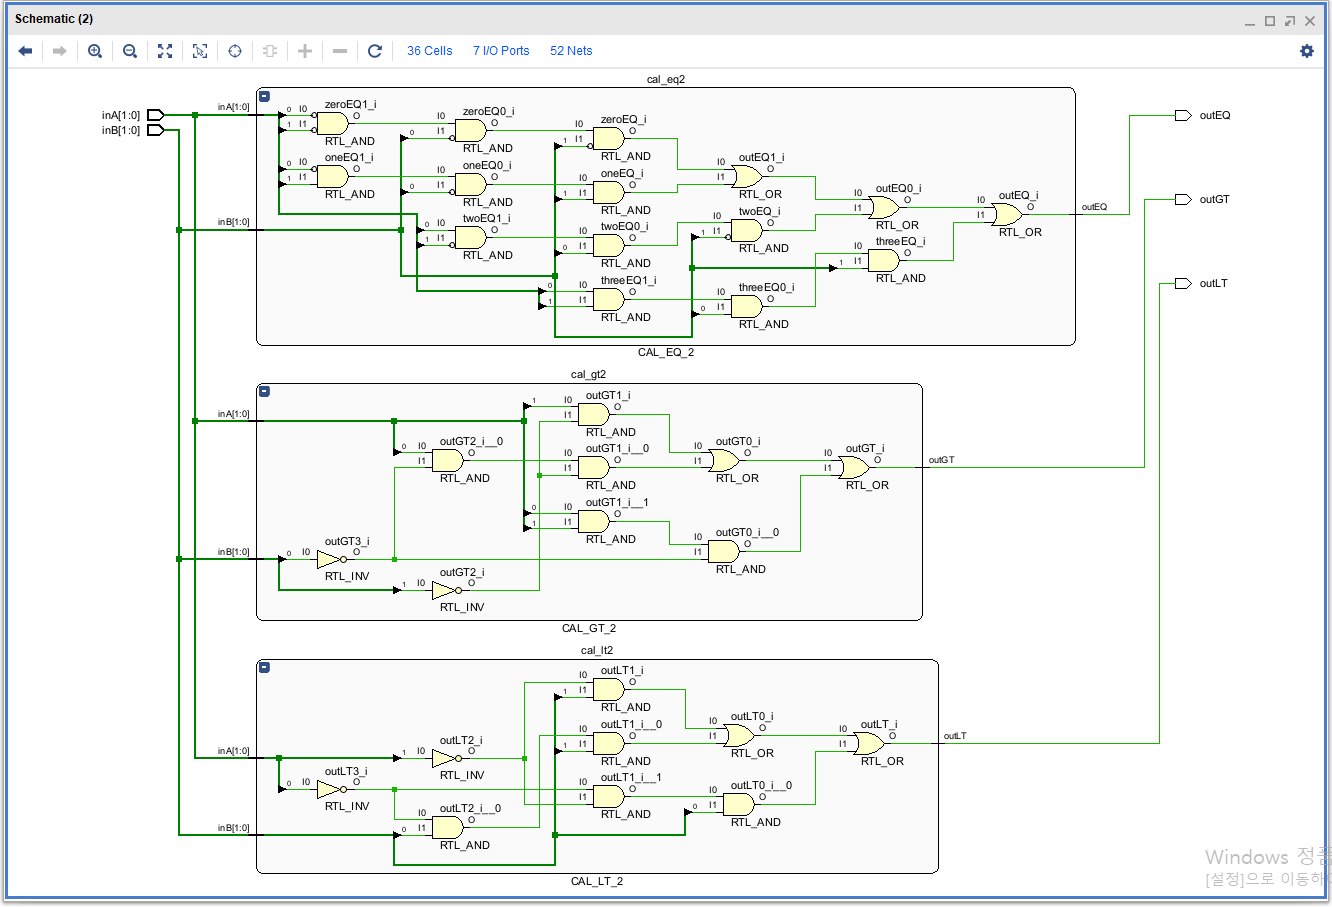
\includegraphics[width=\linewidth]{lab2_2_schematic}
\end{figure}
Netlist는 다음과 같다.
\begin{figure}[H]
  \centering
  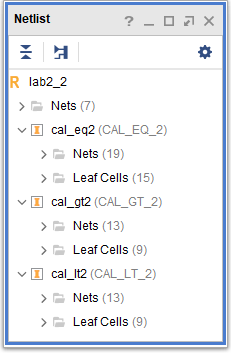
\includegraphics[width=0.4\linewidth]{lab2_2_netlist}
\end{figure}

\(A = B\)를 계산하는 회로는 simplification을 더 이상 할 수 없기 때문에 wire, gate 개수가 두 경우 모두 19, 15개이지만, \(A < B\), \(A > B\)를 계산하는 회로는 simplification 이후 wire, gate 개수가 모두 각각 23, 19개에서 13, 9개로 개수가 감소한 것을 알 수 있다.

과제에 명시적으로 나와 있지는 않았지만, 간단한 테스트벤치를 작성하여 설계한 회로의 정상 작동도 확인해 보았다. 다음과 같은 테스트벤치 코드를 작성하였다.
\lstset{language=Verilog}
\begin{lstlisting}
`timescale 1ns / 1ps

module lab2_tb();
    wire outGT1, outEQ1, outLT1, outGT2, outEQ2, outLT2;
    reg [1:0] A, B;

    lab2_1 cmp1(outGT1, outEQ1, outLT1, A, B);
    lab2_2 cmp2(outGT2, outEQ2, outLT2, A, B);

    initial begin
        A = 2'b00;
        B = 2'b00;
        #16 $finish;
    end

    always begin
        #8 A[1] <= !A[1];
    end

    always begin
        #4 A[0] <= !A[0];
    end

    always begin
        #2 B[1] <= !B[1];
    end

    always begin
        #1 B[0] <= !B[0];
    end
endmodule
\end{lstlisting}

테스트벤치를 실행해 얻은 파형은 다음과 같다.
\begin{figure}[H]
  \centering
  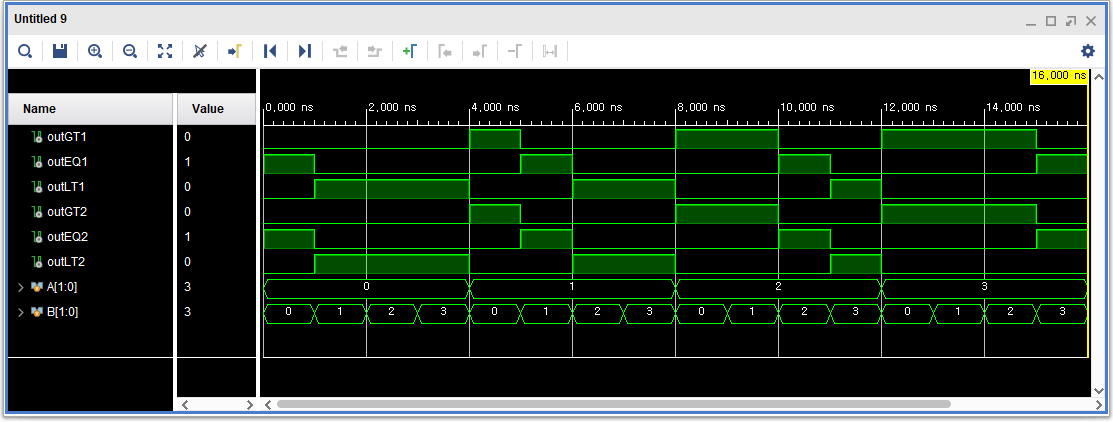
\includegraphics[width=\linewidth]{lab2_waveform}
\end{figure}

\texttt{A}와 \texttt{B} 레지스터는 각각 0으로 시작해서 \texttt{A[1]}은 8ns, \texttt{A[0]}은 4ns, \texttt{B[1]}은 2ns, \texttt{B[0]}은 1ns마다 비트를 뒤집는 방식으로 코딩하였다. 파형에서 볼 수 있듯 \texttt{A}는 16ns를 주기로 0, 1, 2, 3을 순환하고, \texttt{B}는 4ns를 주기로 0, 1, 2, 3을 순환한다.
파형에서 나온 것과 같이, \texttt{A}와 \texttt{B}의 비교 결과가 \texttt{outGT1}, \texttt{outEQ1}, \texttt{outLT1}와 \texttt{outGT2}, \texttt{outEQ2}, \texttt{outLT2}에서 나오는 것을 알 수 있다.

\section{논의}
이 실험을 통해 2bit magnitude comparator를 구현하고 시뮬레이션해 볼 수 있었다. 특히 \texttt{lab2\_1.v}를 작성할 때에 반복적으로 나오는 코드가 있었는데, 이 부분에서 코딩 실수가 많았다. 베릴로그 코드를 수동으로 고치는 것이 힘들어 다음과 같은 파이썬 코드를 작성하여 베릴로그 코드 생성을 자동화하는 경험도 할 수 있었다. 다음은 사용했던 코드의 일부인데, \(A < B\)인 경우를 처리하는 부분의 베릴로그 코드를 생성한다.
\lstset{language=Python}
\begin{lstlisting}
import itertools

for a0, a1, b0, b1 in itertools.product(range(2), repeat=4):
    if (a1, a0) >= (b1, b0):
        continue
    minterm_id = a0 * 8 + a1 * 4 + b0 * 2 + b1
    negs = [('~', ' ')[x] for x in (a0, a1, b0, b1)]
    expr = f"{negs[0]}inA[0] & {negs[1]}inA[1] & {negs[2]}inB[0] & {negs[3]}inB[1]"
    print(f"assign min{minterm_id:04b} = {expr};")
\end{lstlisting}
K-map을 사용한 대수식의 simplification 뿐만 아니라, 정확한 코드를 쉽게 작성할 수 있는 방법에 대한 고민도 할 수 있는 시간이었다.

\end{document}
